\documentclass[a4paper,12pt]{report}

\usepackage{alltt, fancyvrb, url}
\usepackage{authblk}
\usepackage{graphicx}
\usepackage{subfigure}
\usepackage{wrapfig}
\usepackage{algorithmic}
\usepackage[utf8]{inputenc}
\usepackage{fontenc}
\usepackage{amsmath,stmaryrd,mathtools,algorithm}
\usepackage{amssymb}
\usepackage[document]{ragged2e}
\usepackage[italian]{babel}
\usepackage{hyperref}

\title{\Huge \textbf{Relazione Progetto OOP}}
 
\author{Giulianini Andrea, Lombardi Alessandro, Meluzzi Marco, Stockman Alessandro}
\date{\today}


\begin{document}
 
\maketitle
\justify

\tableofcontents

\chapter{Analisi}

\section{Requisiti}

Il programma qbert è un remake del videogioco arcade Q*Bert pubblicato nel 1982 dalla  Gottlieb. In altri termini si tratta di un rifacimento che  tende a ricostruire abbastanza  fedelmente, se non tutte, almeno le principali caratteristiche del gioco originale.

\subsubsection{Requisiti funzionali}
\begin{itemize}
	\item Il giocatore servendosi degli appositi input da tastiera, può muovere il personaggio principale in quattro direzioni. Lo scopo di ogni round, con i quali si articola il gioco, è colorare gradualmente la faccia superiore di ciascun cubo della mappa piramidale di un certo colore.
	\item Il numero di colori e i colori stessi che un cubo può assumere possono variare da un livello all'altro. Esiste inoltre la possibilità di ricominciare a ciclare il set colori disponibili una volta raggiunto l'ultimo, rendendo di fatto più complesso l'obiettivo del gioco.
	\item Nel gioco sono presenti vari personaggi, l'interazione fra il protagonista e questi avviene tramite contatto, alcuni di questi sono amici, quindi possono favorire il protagonista nel raggiungimento del suo obiettivo, altri sono nemici. Generalmente i nemici sono da evitare, in quanto una collisione con questi sarebbe letale per il protagonista, ma vi sono altri che possono essere eliminati. I personaggi possono avere movimenti e comportamenti differenti.
	\item I movimenti possono andare dall'alto verso il basso, terminando a seconda del personaggio specifico con una caduta fuori dalla mappa oppure con movimenti più intelligenti e tendenti ad inseguire il giocatore.
	\item Dal punto di vista dell’ambiente di gioco, questo deve adattarsi consistentemente all’avanzamento dello stesso, in modo da rispecchiare la struttura a livelli prevista e il graduale aumento della difficoltà del gameplay.
	\item Il vero scopo del giocatore è sopravvivere e ottenere punteggi elevati. E' possibile guadagnare punti in diversi modi durante il corso della partita.
\end{itemize}

\subsubsection{Requisiti non funzionali}
\begin{itemize}
	\item Realizzazione di una grafica molto simile a quella originale ma più moderna
	\item Garantire la fluidità dell’esperienza di gioco

\end{itemize}

\section{Analisi e modello del dominio}

Il programma deve gestire una sessione di gioco composta da vari livelli, certe informazioni si mantengono da un livello all'altro, ad esempio le vite del protagonista oppure il punteggio accumulato, mentre altre saranno ogni volta ricalcolate. Un livello presenta elementi "statici", come la natura dei cubi di cui è composto, e "dinamici", come il set di antagonisti che si possono incontrare. Il livello si occupa della creazione e aggiornamento del terreno di gioco gestendo gli oggetti statici presenti,  dell'aggiornamento del punteggio causato da differenti eventi e del controllo della corretta esecuzione delle regole del gioco. Il livello interagisce con un'altra entità, detta Spawner, per controllare che la quantità dei personaggi in azione sia adatta al livello di difficoltà raggiunto. Il ciclo di vita dei personaggi è spesso breve e semplice, essi eseguono una serie di movimenti personalizzati e indipendenti, mentre interagiscono con l'ambiente esterno quasi univocamente tramite collisione.

Fra le difficoltà che si potrebbero incontrare potrebbe esserci quella di costruire un dialogo livello-personaggi-spawner in modo da mantenere una certa indipendenza tra le entità e una suddivisione chiara dei ruoli. Il requisito non funzionale sulla giocabilità del software finale richiederà molte prove e una certa dose di abilità di game design, quindi sarà fatto verso la fine e potrà essere accorciato per motivi di tempo.

\begin{figure}[H]
\centering{}
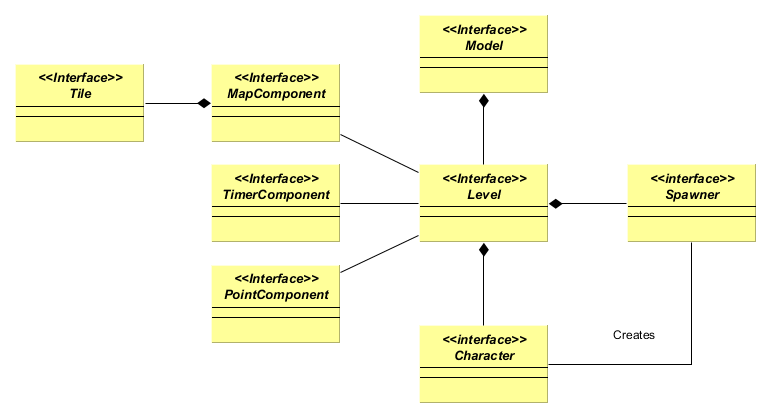
\includegraphics[width=\linewidth]{img/Analisi}
\caption{Schema dell'analisi e modello del dominio}
\label{img:Analysis}
\end{figure}

\chapter{Design}

\section{Architettura}

L'architettura dell'applicazione è realizzata utilizzando il pattern architetturale MVC in quanto permette facilmente di separare la logica e i dati della applicazione dalla effettiva tecnica adottata per la visualizzazione di questi. La applicazione e quindi la relativa architettura sono suddivise in varie implementazioni a seconda dello stato nelle quali si trovano.

L'interfaccia Model fornisce tutte le funzionalità comuni ad ogni stato della applicazione per comunicare al Controller i dati da mostrare e presentare i comandi capace di ricevere e in grado di influenzare l'esecuzione della logica interna. La gestione dello stato corrente e la relativa implementazione lato model è fatta da una entità preposta del Controller detta GameStatusManager. 

\begin{figure}[H]
\centering{}
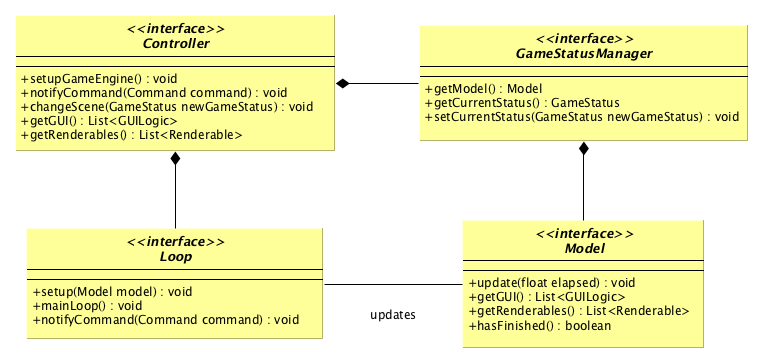
\includegraphics[width=\linewidth]{img/ArchitetturaControllerModel}
\caption{Il dialogo fra Controller e Model}
\label{img:ControllerModel}
\end{figure}

Il Controller si occupa principalmente di gestire il dialogo fra Model e View, oltre che di fornire numerose funzionalità per la lettura e scrittura su file di dfferenti tipi di dati persistenti. Il Controller deve inoltre gestire una componente vitale della applicazione detta Loop, che permette di aggiornare la grafica e la logica di gioco nel tempo, sostituendo il Model quando cambia lo stato del programma.

Il dialogo fra Controller e View è più stabile in quanto è la View stessa ad associare alle differenti scene lo stato di gioco e di realizzare effettivamente il cambio da una scena all'altra. Scene svolge effettivamente la renderizzazione grafica sfruttando particolari classi, aggiornate dal Model, che confezionano tutti i dati necessari per disegnare correttamente immagini (Renderable) e GUI (GUILogic).

\begin{figure}[H]
\centering{}
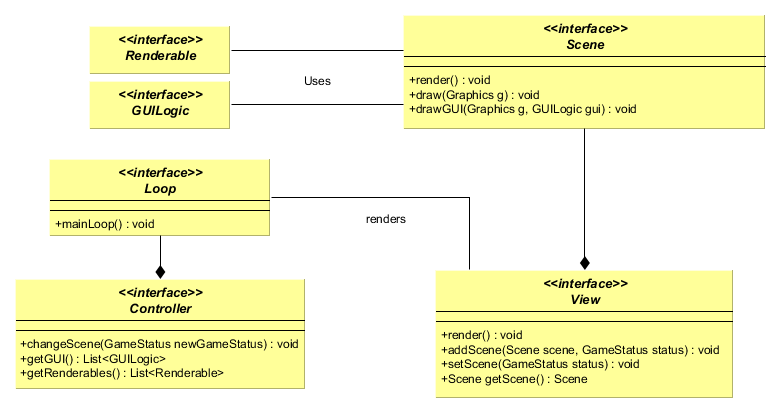
\includegraphics[width=\linewidth]{img/ArchitetturaControllerView}
\caption{Il dialogo fra Controller e View}
\label{img:ControllerView}
\end{figure}

\section{Design dettagliato}

\begin{flushright}
\item\subsubsection{Alessandro Lombardi - Logica dei personaggi}
\end{flushright}

I personaggi svolgono diverse azioni e fanno diverse scelte durante il loro ciclo di vita. Per evitare una gestione troppo cablata e poco mantenibile delle specifiche situazioni è stato scelto di utilizzare lo \textbf{State Pattern}. Il pattern State evita l'utilizzo di monolitici  blocchi condizionali all'interno delle classi dei singoli personaggi per la scelta e l’esecuzione di una azione piuttosto che un’altra, frammentando lo svolgimento delle singole azioni a classi specifiche che sono riutilizzabili e facilmente intercambiabili tra loro. Inoltre, permette di gestire meglio l'esecuzione delle animazioni e la simulazione delle attese che un personaggio fa fra un'azione e l'altra. Nella pratica ogni personaggio viene aggiornato col passare del tempo tramite il metodo update(float dt), ma questo delega completamente i propri compiti allo stato attuale.

Nel caso specifico  è stato scelto di associare a ciascun personaggio uno stato di riposo, reperibile tramite il metodo getStandingState() presente della interfaccia \emph{Character}, caratteristico per ciascuno e paragonabile a uno stato di attesa di una macchina a stati finiti responsabile delle maggiori scelte logiche del personaggio, come la strategia di movimento. La classe astratta \emph{CharacterStateImpl} è una semplice implementazione dell'interfaccia \emph{CharacterState} e viene ereditata direttamente dagli stati molto semplici o di transizione, come rispettivamente \emph{QbertStandingState} e \emph{LandState}. Le classi astratte \emph{WaitAnimationState} e \emph{WaitTimerState} invece, usano il metodo update() come \textbf{Template Method} per permettere alle classi concrete la personalizzazione nel metodo conclude() delle azioni da svolgere, rispettivamente alla fine di una animazione o allo scadere di un timer. \emph{MoveState} contiene gli stati usati da tutti i personaggi per eseguire i basilari movimenti nelle due o quattro direzioni a seconda del tipo di \emph{Character} che viene passato. 

\begin{figure}[H]
\centering{}
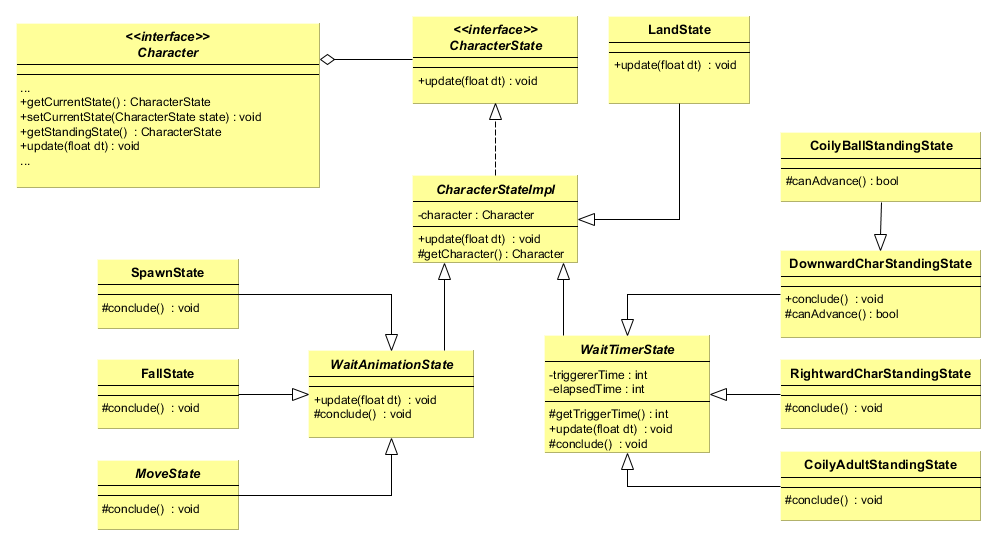
\includegraphics[width=\linewidth]{img/CharacterStates}
\caption{Alcune delle principali classi della gerarchia dei Character State}
\label{img:CharacterStates}
\end{figure}

E' importante sottolineare che gli stati vengono inizializzati passando il \emph{Character} associato, permettendo allo stato di applicarvi le modifiche necessarie, quindi i costruttori degli stati sono modellati per accettare anche le classi più specifiche della gerarchia dei personaggi, limitando e proteggendo gli stati che devono essere usati solo per certi personaggi. Ad esempio, \emph{QbertOnDiskState} accetta solo \emph{Player}, mentre \emph{FallState} può accettare un \emph{Character} oppure un \emph{DownUpwardCharacter} personalizzando le azioni da compiere di caso in caso.


\begin{figure}[H]
\centering{}
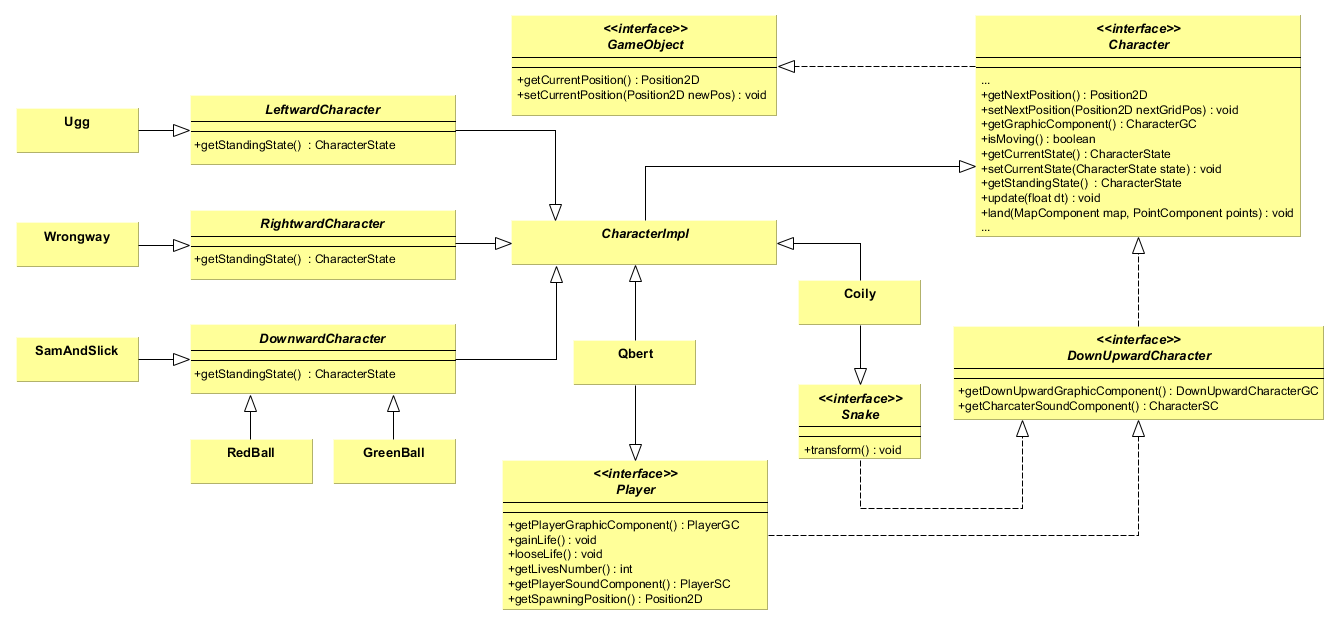
\includegraphics[width=\linewidth]{img/GerarchiaCharacters}
\caption{La gerarchia dei Character}
\label{img:GerarchiaCharacters}
\end{figure}

\begin{flushright}
\item\subsubsection{Alessandro Lombardi - Animazione dei personaggi}
\end{flushright}

Durante la fase di analisi è stato scelto di dividere quella che era la posizione "logica" del personaggio, ovvero la posizione nella griglia immaginaria disegnata dalle facce dei cubi del terreno di gioco, da quella "fisica", ovvero la coordinata del pixel nella finestra di gioco, dove si posiziona l'angolo in alto a sinistra dell'immagine di forma rettangolare del personaggio. Questo ha comportato anche una divisione degli aspetti grafici da quelli logici e la scelta di considerare i movimenti come il salto, la caduta etc.. vere e proprie animazioni. La gestione dei dati necessari alla renderizzazione grafica dei personaggi, quali la posizione, lo sprite e la dimensione di questo, sono gestiti dalle classi che implementano \emph{CharacterGC}. La gerarchia dei Character Graphic Component si basa sul riutilizzo del codice in comune e sulle animazioni supportate, \emph{CharacterGC} fornisce i metodi per la gestione delle animazioni e presenta quelle base. Le interfacce e le classi per la gestione della grafica di Coily e Qbert supportano animazioni per muoversi anche verso l'alto oltre che gestire gli sprite per il fronte e il dietro dei personaggi. Da notare come Coily sfrutti il metodo setFrontSprites(OneSideCharacterSprites frontSprites) per trasformarsi dalla palla viola che è inizialmente alla sua forma finale.

\begin{figure}[H]
\centering{}
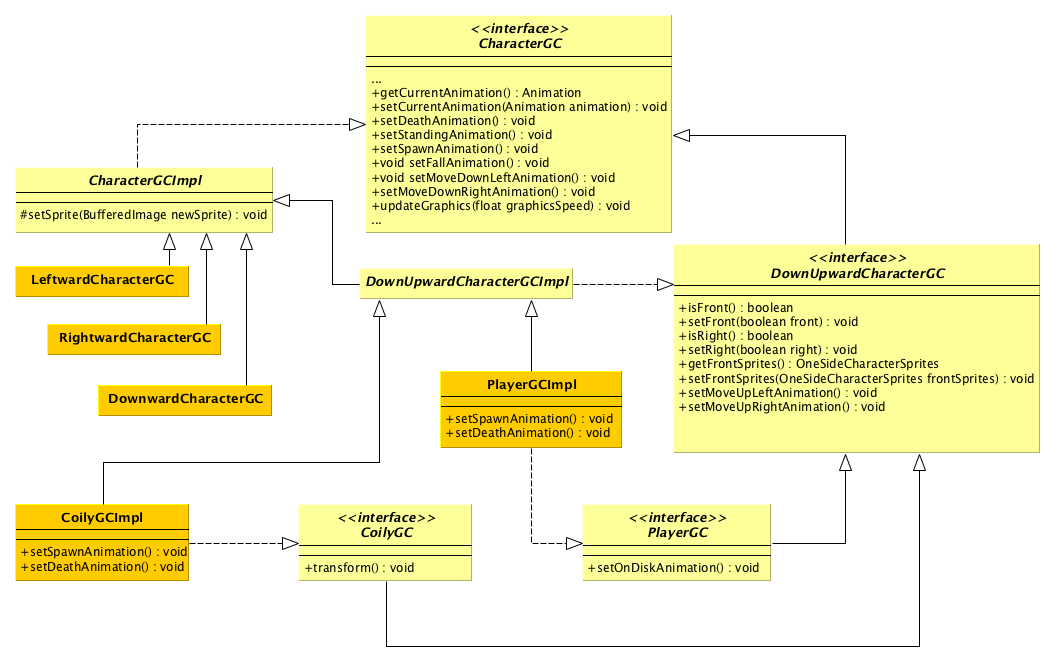
\includegraphics[width=\linewidth]{img/GerarchiaCGC}
\caption{La gerarchia CharcaterGC}
\label{img:GerarchiaCGC}
\end{figure}

Le animazioni dei personaggi sono state sviluppate sfruttando il pattern \textbf{Iterator} essendo queste delle sequenze di posizioni bidimensionali nella finestra di gioco e/o di immagini. La interfaccia \emph{Animation} nasconde le modalità di scorrimento e le condizioni di termine dell’animazione, richiedendo però dettagli sulla velocità di esecuzione. L’implementazione \emph{MovementAnimation} di \emph{Animation} è particolarmente specifica per quelle animazioni basate sul movimento della posizione dell'immagine. \emph{MovementAnimation} è una classe astratta che contiene l’implementazione di molti metodi utili per le animazioni di movimento ma che lascia alle classi concrete l’effettiva decisione del calcolo delle posizioni, tramite il metodo calculateNext() invocato nel \textbf{Template Method} updateAnimation(float animationSpeed). \emph{ComposedAnimation} permette di costruire animazioni più complesse formate da singole semplici animazioni.

\begin{figure}[H]
\centering{}
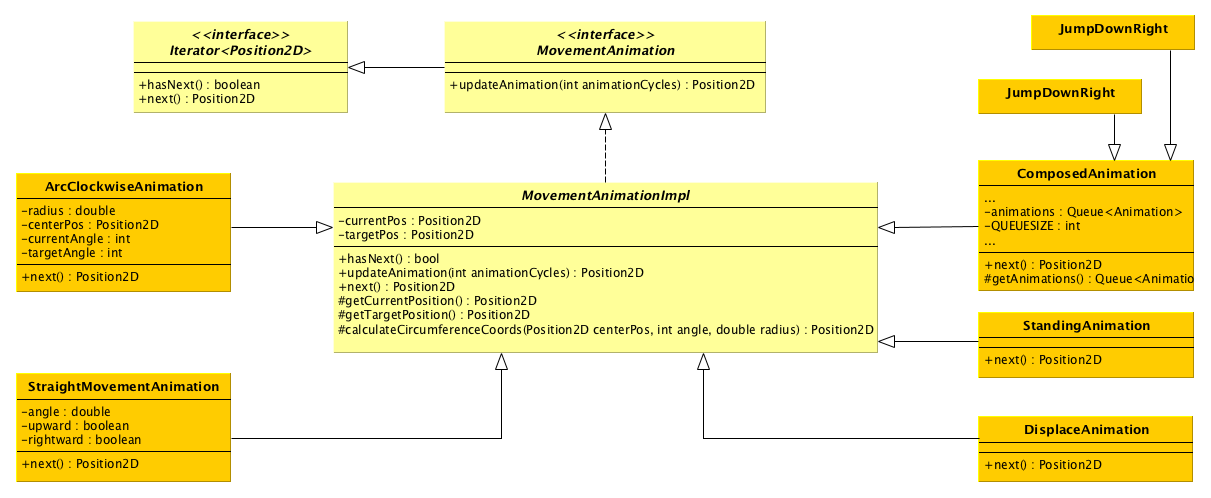
\includegraphics[width=\linewidth]{img/AnimazioniPersonaggi}
\caption{Alcune animazioni dei characters}
\label{img:AnimazioniPersonaggi}
\end{figure}


\chapter{Sviluppo}
\section{Testing automatizzato}


\section{Metodologia di lavoro}

La suddivisione del lavoro è stata concepita con lo scopo di lasciare molta indipendenza fra i componenti del gruppo, nel rispetto dei tempi e degli impegni di ciascuno. Dopo una prima fase di analisi utile soprattutto a definire il dominio e confermare la suddivisione del lavoro, si è cercato di produrre un prototipo funzionante che permettesse la gestione dei movimenti e delle collisioni dei primi personaggi. La scelta e la implementazione del loop di gioco è stata fatta assieme, mentre ciascuno ha poi proseguito indipendentemente nel proprio lavoro, non mancando mai a comunicare, chiedere anche solo consigli al resto del gruppo. La parte di Model è stata predominante durante questa fase di sviluppo, concentrando il gruppo principalmente nella realizzazione sempre più dettagliata del gioco, includendo pian piano tutte le regole, i personaggi fondamentali e la gestione del punteggio. Con il Model pressochè ultimato e la necessità di aggiungere altre funzionalità alla applicazione si è ampliato la parte di Controller relegato al controllo del game loop alla gestione di più schermate con l'introduzione di scene e parti di View fino a quel momento ignorate nella implementazione. In generale lo sviluppo è stato un processo a spirale dovuto non solo alle correzioni e i miglioramenti architetturali e di dettaglio del codice ma anche alle tempistiche diverse dei membri del gruppo che seppur autonomi si sono mantenuti paralleli.
Nello specifico la divisione dei compiti è stata la seguente:
\begin{itemize}
	\item \textbf{Giulianini Andrea}:

	\item \textbf{Lombardi Alessandro}: Realizzazione dei personaggi, sia negli aspetti grafici, animazioni e sprites, che in quelli logici, comportamento e strategia di movimento. Gestione dialogo model-view per la gestione della GUI, incapsulamento delle informazioni lato model, come testo e selezione, stilizzazione e formattazione lato view a seconda della parte di pagina occupata. Disegno degli sprites in formato vettoriale.

	\item \textbf{Meluzzi Marco}:

	\item \textbf{Stockman Alessandro}:

\end{itemize}

\section{Note di sviluppo}

	\item \textbf{Giulianini Andrea}:

	\item \textbf{Lombardi Alessandro}: Nello sviluppo delle animazioni e poi successivamente della GUI ho approfondito alcuni aspetti non trattati a lezione circa il funzionamento con il quale swing e awt effettuano il "painting" e la possibile personalizzazione di questo per la nostra applicazione. Sempre nella gestione della GUI ho fatto uso della classe Optional per controllare la presenza o meno nelle varie scene delle implementazioni lato view delle parti di una finestra (\emph{Optional<GUISection>}) e del font. Per il posizionamento centrale delle stringhe basato sulla grandezza della finestra e del font mi sono rivolto a chi lo aveva fatto prima di me (\href{https://stackoverflow.com/questions/27706197/how-can-i-center-graphics-drawstring-in-java}{link}). Ho sfruttato l'API fornita da Java per la gestione di un minimale sistema di logging su file XML o su console, per scopi di debug ma anche segnalazione di errori  fatali per la applicazione.

	\item \textbf{Meluzzi Marco}:

	\item \textbf{Stockman Alessandro}:

\chapter{Commenti finali}


\section{Autovalutazione e lavori futuri}


\section{Difficoltà incontrate e commenti per i docenti}


\appendix
\chapter{Guida utente}


%\bibliographystyle{abbrv}
%\bibliography{template}

\end{document}